\subsection{Camera internal matrixes}

The camera consists of Intrinsic and extrinsic parameters,
K * [R | T]
The extrinsic parameters consists of a 3x3 rotation matrix (R )and a
translation vector (T). The translation vector expresses the origin of the world
coordinate system in camera coordinates. 
These transforms the coordinates from 3d world coordinates to 3d camera
coordinates. 

The intrinsic matrix (K) contains 5 parameters.

\begin{figure}[!htbp]
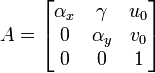
\includegraphics{pics/intristic_parameters.png}
\caption{Intrinsic/camera -matrix (here represented by "A")}
\label{fig:intrinsic_parameters}
\end{figure}

Alpha-X = focal length * scale factor(for x-coords), and 

Alpha-Y = focal length * scale factor(for y-coords). These converts real world
length (in mm) to pixel distance. 

$\gamma$  is the skew coefficient, and u0 v0 are the camera center.
